\documentclass{report}

% Page Size
\usepackage[letterpaper, portrait, margin=1in, left=1.5in]{geometry}

% Spacing
\usepackage{setspace}
\setlength{\parskip}{\baselineskip}
\doublespacing{}


% Bibliography
\usepackage[american]{babel}
\usepackage[style=apa, citestyle=apa, backend=biber]{biblatex}
\DeclareLanguageMapping{american}{american-apa}
\addbibresource{references.bib}
\usepackage[babel,threshold=2]{csquotes}

% Graphics
\usepackage{graphicx}
\graphicspath{ {./images/} }

% Table of Content
\setcounter{tocdepth}{2}

% Code Formatting
\usepackage{minted}
\usemintedstyle{pastie}

\def\code#1{\texttt{#1}}

% Positioning
\usepackage{float}

% Acronyms
\usepackage{acro}

\DeclareAcronym{iso}{
	short=ISO,
	long=International Organization for Standardization
}

\DeclareAcronym{ansi}{
	short=ANSI,
	long=American National Standards Institute
}

\DeclareAcronym{jis}{
	short=JIS,
	long=Japanese International Standards
}

\DeclareAcronym{wpm}{
	short=WPM,
	long=Words per Minute
}

\DeclareAcronym{neck}{
	short=WRNULD,
	long=Work-related neck and upper limb disorders
}

\DeclareAcronym{cv}{
	short=CV,
	long=Computer Vision
}

% Chapter Formatting
\usepackage{titlesec}
\titleformat{\chapter}[display]
{\centering\LARGE\normalfont\bfseries}
{Chapter \thechapter}
{0em}
{\vspace{-1.5ex}}

% Colors
\usepackage[dvipsnames]{xcolor}

% Links
\usepackage{hyperref}
\hypersetup{
	pdftitle={Development of a touch typing trainer with an emphasis on finger and wrist placement},
	pdfstartview={FitH},
	colorlinks=true,
	linkcolor=black,
	citecolor=black,
	filecolor=black,
	urlcolor=MidnightBlue
}


\begin{document}

\pagenumbering{gobble}
\begin{titlepage}
	\centering

	\hspace{0pt}
	\vfill

	
\includegraphics[width=0.2\textwidth]{upc.png}
	
\includegraphics[width=0.2\textwidth]{dcs.png}
	\par\vspace{1cm}

	\textsc{Development of a touch typing trainer\\with an emphasis on finger and wrist positions}
	\par\vspace{0.5cm}

	\hrulefill
	\par\vspace{0.25cm}
	A Special Project Proposal Presented to the\\
	Faculty of the Department of Computer Science,\\
	University of the Philippines Cebu

	\par\vspace{0.25cm}
	In Partial Fulfillment\\
	Of the Requirements for the Degree\\
	Bachelor of Science in Computer Science\\
	\par\vspace{0.25cm}
	\hrulefill
	\par\vspace{0.5cm}

	Oscar Vian L. Valles\\
	BS Computer Science
	\par\vspace{0.5cm}

	Dhong Fhel K. Gom-os\\
	Adviser
	\par\vspace{0.5cm}

	October 2021
	\vfill
	\hspace{0pt}
\end{titlepage}
\newpage


\printacronyms
\newpage

\tableofcontents
\newpage

\pagenumbering{arabic}

\chapter{Introduction}


%FIXME - Lots of passive voice
\section{Background of the Study}
There are a lot of educational typing tests available that help people learn
touch typing, including Monkeytype, TypeRacer, and Keybr. These typing tests list
out words that are then typed out. The inputted keys are then compared to check
if the user has typed the expected letter. At the end of the test, the time
taken is calculated, and certain metrics are given. These metrics include words
per minute (WPM) and accuracy \parencite{bartnik2021}.

However, this method of examination leaves out a crucial part of typing —
ergonomics. Ergonomic typing prevents a lot of health issues in the future like
repetitive strain injury or carpal tunnel. One important factor that affects
ergonomics is the typing procedure and posture. This means the proper placement of
the wrist, hands, and hitting the keys using the right finger that is assigned
to the key.

Correct finger placement is usually taught at the beginning using a diagram,
with each key being associated with a specific finger. For instance, the letter
Q in a QWERTY layout should be hit using the fifth digit of the left hand, and
this is shown by coloring the fifth digit and the key Q with the same color or
by placing the letters directly on the fingers \parencite{dobson2009touch}.

Incorrect finger placement may cause these hand and wrist positions: ulnar
deviation, forearm pronation, and wrist extension \parencite{serina1999}. These
three are hand and wrist positions that are common in all activities, however,
prolonged periods in these positions may cause injuries such as Carpal
tunnel syndrome (CTS) \parencite{toosi2015}

In addition, this type of typing is frequently taught in the beginner level
\parencite{donica2018}. This means that there is a need to weed out bad habits
that may develop, like using the index finger for pressing the spacebar or
backspace. However, it is impractical for an educator to check each student if
they are not performing these movements as these may only show for a small
period which may not be caught in time.

Thus, there is a need for automatically detecting which finger is used during
typing, and for the position of the wrist in relation to the arm. One way to do
this is through finger and hand tracking. One solution for tracking is by using
image processing and machine learning. An example of this is MediaPipe
by~\cite{mediapipe}.

MediaPipe allows for various applications for machine learning in the field of
image processing. This includes, hand tracking, pose estimation, object
detection, and others. Another example of a library that allows for hand and
finger tracking is OpenCV by~\cite{opencv}. This is a tool that simplifies
computer vision and image processing. Machine learning can also be used with
OpenCV.

\section{Research Objectives}

\subsection{General Objectives}
To create a touch typing trainer that detects poor finger placement and hand
position to help develop better typing habits and healthier typing ergonomics.

\subsection{Specific Objectives}
\begin{itemize}
	\item To develop a program that tracks fingers and hand positions while typing
	\item To create a subroutine that ascertains which finger was used to type a key
	\item To detect if incorrect fingers were used to press a key or if the
	      position of the hand in relation to the wrist is problematic
	\item To assess the accuracy and performance of the developed program's ability
	      to perform the previously stated objectives
	\item To develop a user-friendly interface for users to train touch typing
	      using the developed program
	\item To generate key statistics of a user's touch typing performance:
	      \begin{itemize}
		      \item Words per Minute
		      \item Accuracy
		      \item Finger Placement Accuracy
	      \end{itemize}
\end{itemize}


\section{Scope and Limitation}
This research will focus on typing on a 60\% keyboard. Figure~\ref{fig:60}
illustrates this type of keyboard. This type of keyboard only has the
alphanumeric part of the keyboard. This limits the number of keys to be checked
and the expected movement of the hand. Furthermore, the keycaps will also be of
a light color, while the surface that the keyboard rests upon will be of a dark
color.

In addition, the keyboard layout will be \ac{ansi}. This layout is described by the
American National Standards Institute \parencite{ansi}. This is the most
common layout in the United States. However, it is also used in numerous
English-speaking countries such as the Philippines, Malaysia, and India.

The program will expect the that user has all ten digits and has no hand,
finger, or wrist deformities. In addition, only the placement of the hands,
fingers, and wrists will be taken into account when determining if the
ergonomics of the user while typing is healthy. The program will not check
seating position, angle of elbows, and other metrics for an ergonomic typing
posture while typing.

Capturing of the video to be analyzed by the program would be limited to a
single 1080p webcam that is capturing in 60 frames per second. The camera will
be pointed downwards facing the keyboard and the hand. This means that the
vertical angle of the wrist may not be accurate.

\begin{figure}[H]
	\centering
	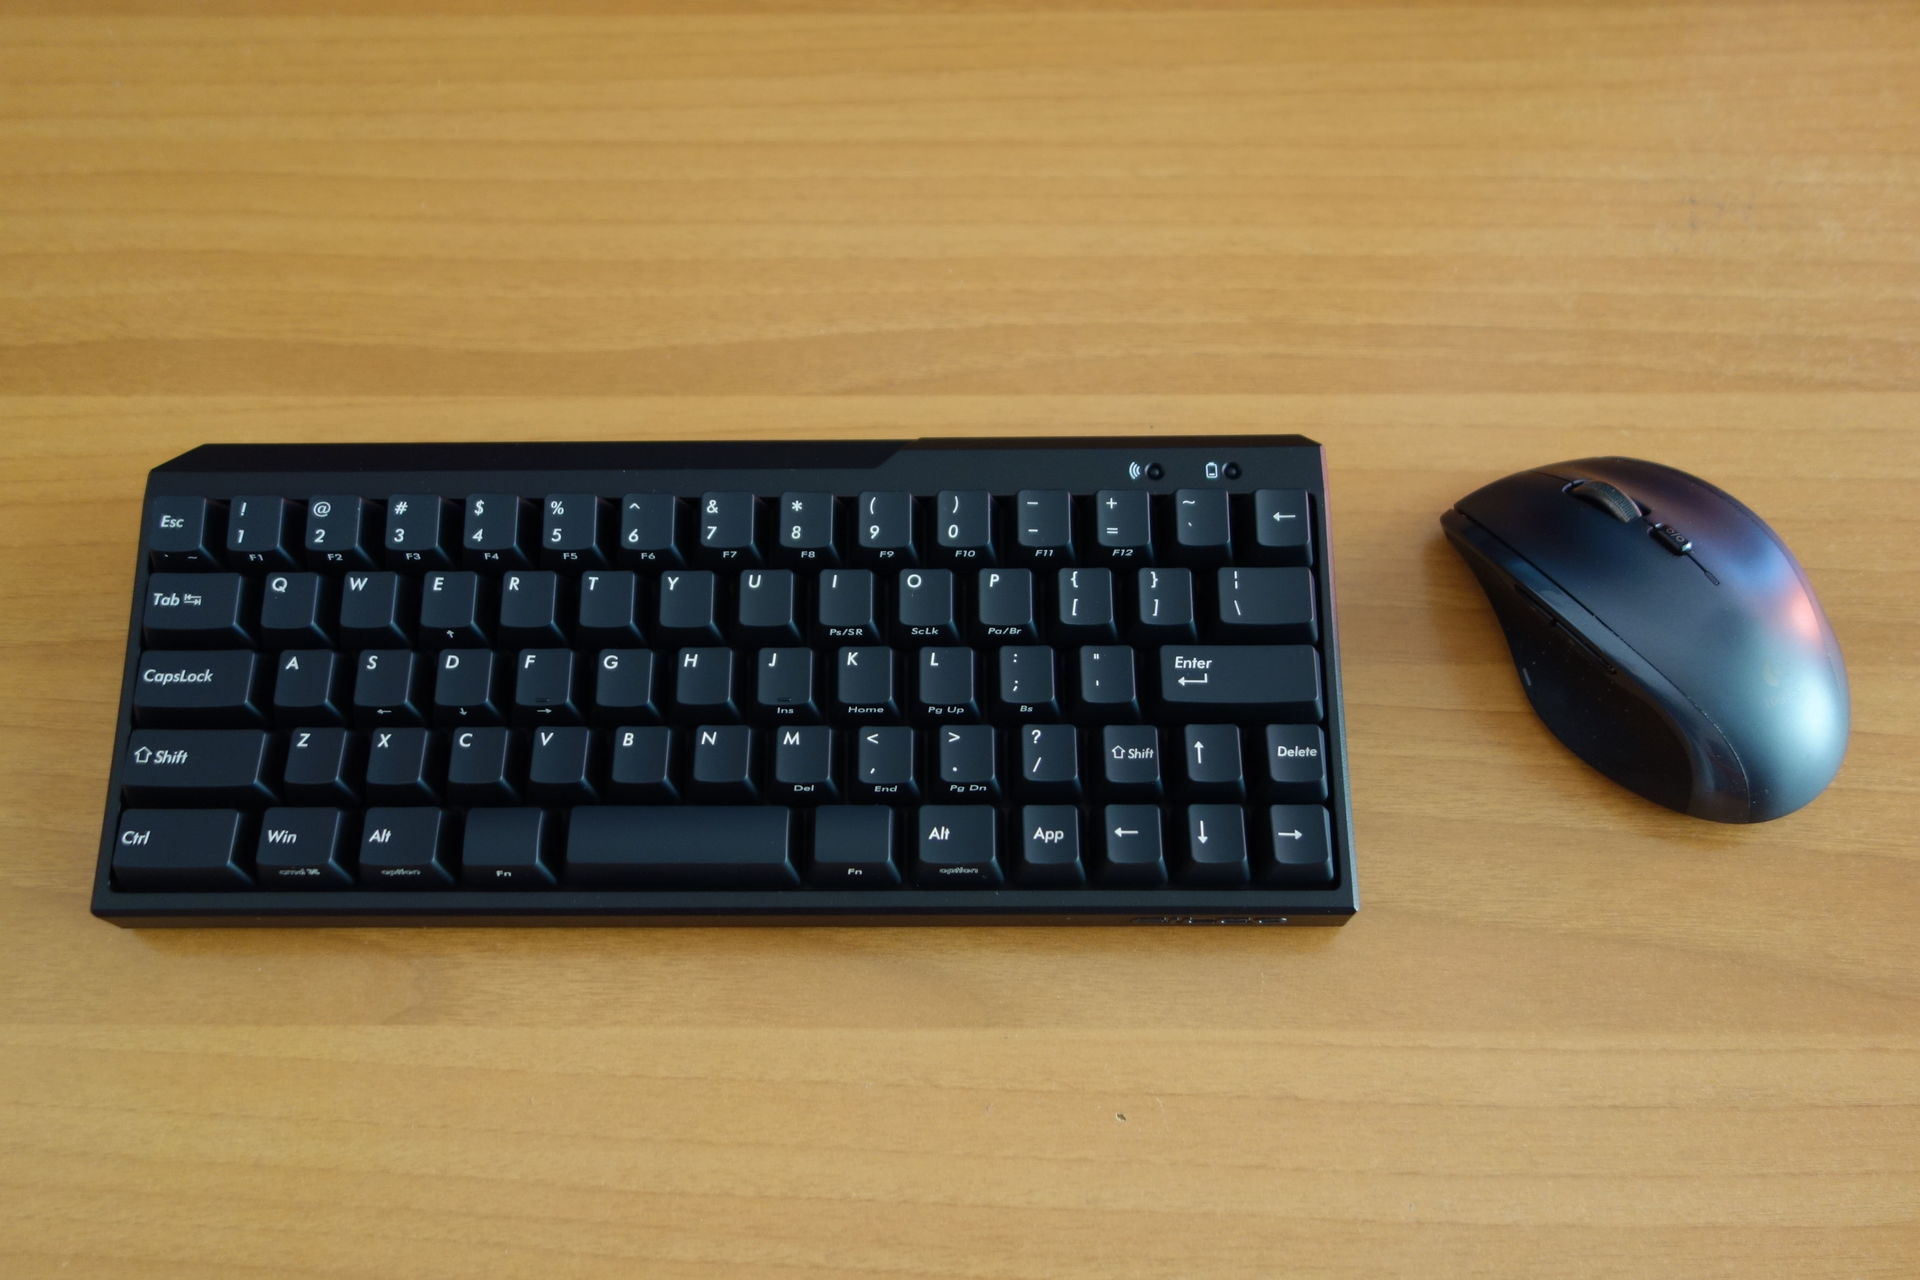
\includegraphics[width=0.8\textwidth]{60.jpg}
	\caption{A 60\% keyboard in \ac{ansi} layout. Reprinted from \fullcite{60}}
	\label{fig:60}
	\centering
\end{figure}


\section{Significance of the Research}
This research is beneficial for all users of physical keyboards. These include a
vast majority of the population as there are a lot of professions that heavily
rely on keyboards. Examples include developers, physicians, educators,
accountants. By having better ergonomics while typing, wrist injuries can be
prevented, and typing speed may be increased

This research also helps educators, especially early educators teaching beginner
typists. By automatically checking for ergonomics, posture, and correct
technique, the burden of checking each student is lessened, and directed
interventions for bad habits can be easily created as students with these bad
habits are easily identified

This research has a direct impact on people that has hand or wrist injuries that
are caused by poor typing habits. By correcting these poor habits, pain from
these injuries will be lessened, and even be prevented from occurring in the
first place. A specific example of this is by reducing ulnar deviation which
affects the nerve that is indicative of CTS \parencite{toosi2015}.

\chapter{Preliminary Review of Related Literature}

\section{Keyboard Typing}

Keyboard typing is the process of using a keyboard to input characters in a
system. In the context of this paper, keyboard typing will refer to the act of
using a physical keyboard to input characters in a computer system.

% Insert more about keyboard typing here %

\subsection{Keyboard Layouts and Form Factors}

One key characteristic of a keyboard is its physical attributes. Keyboards come
in a lot of layouts and form factors. Keyboard layouts are the shapes, size, and
positions of a key on a keyboard while the form factor of a keyboard refers to
its shape and dimensions. The form factor also refers to the number of keys included
in the keyboard \parencite{parkkinen2018}. By combining different layouts and
form factors, different permutations of a keyboard can be created.

Different keyboard layouts and form factors also produce different effects for
the user. This is due to how vastly different some keyboard layouts and form
factors are from one another. Some layouts focus on ergonomics, while others
focus on typing speed. Some form factors were designed for aesthetics, while
others focus on comfort and health. As such, different layouts may affect typing
performance, ergonomics, and long-term health effects \parencite{ciobanu2015}.

\subsubsection{ANSI and ISO Layout}

There are two common keyboard layouts around the world --- \ac{iso} and \ac{ansi}.

\citeauthor{ansi} is the standard that first defined the \ac{ansi} layout.
Figure~\ref{fig:ansi} illustrates what the \ac{ansi} layout looks like. This layout
is also used by countries other than America. Examples of countries that use
this layout as its standard is the Philippines, China, and Korea
\parencite{apple-layout}. However, these countries also opt to modify the layout
by adding extra layers to accommodate other character sets.

\citeauthor{iso} is the standard series that defines a framework that is used to
create other layouts. Layouts created from this standard are colloquially called
\ac{iso} Layouts. Countries around the world use this framework to create layouts
that fit the characters in their language. Examples of countries that use this
framework to create their own layout are France, Greece, Canada, and Sweden
\parencite{apple-layout}.

Both of these layouts usually utilize the same key ordering. This ordering is
commonly called QWERTY, based on the first five characters of the first row
of this specific layout.

There are other layouts available, however, they are not as common as the two
previously mentioned layouts. Examples of this include \ac{jis}. Other esoteric
layouts, like Tsangan or split-backspace, also exist. These layouts modify the
\ac{iso} and \ac{ansi} standards by adding or removing certain keys to fit the
character set of a language, or for additional keys. Other layouts are also
exactly the same as \ac{ansi} or \ac{iso}, however, these layouts change the
arrangement of the alphabet within the keyboard.

Despite the ubiquity of these common layouts, studies have shown that these
layouts are not ergonomic. The main issue with these layouts is the random
configurations of the letters. The randomness of the layout necessitates
memorization of the layout which reduces the ease of learning, reduces performance
in typing by reducing speed, and increases of typing errors
\parencite{ciobanu2015}.

\subsubsection{Keyboard Form Factors}

There is only one common keyboard form factor used worldwide: the full-size
keyboard. This keyboard contains all the keys specified in the keyboard
layout. This includes the alphanumeric keys, the function keys, the navigation
cluster, and the numpad.

Other common keyboard form factors are based on the full-size keyboard. The name
of these layouts, 60\%, 75\%, and 80\% reference the remaining number of keys
after cutting a portion off from the full-size keyboard. The 60\% keyboards only
contain the alphanumeric cluster while the 80\% and 75\% layouts retain the
navigation cluster and the function keys \parencite{parkkinen2018}. The main
draw for using keyboards with reduced sizes is for aesthetics, space
constraints, and ergonomics.

\begin{figure}[H]
	\centering
	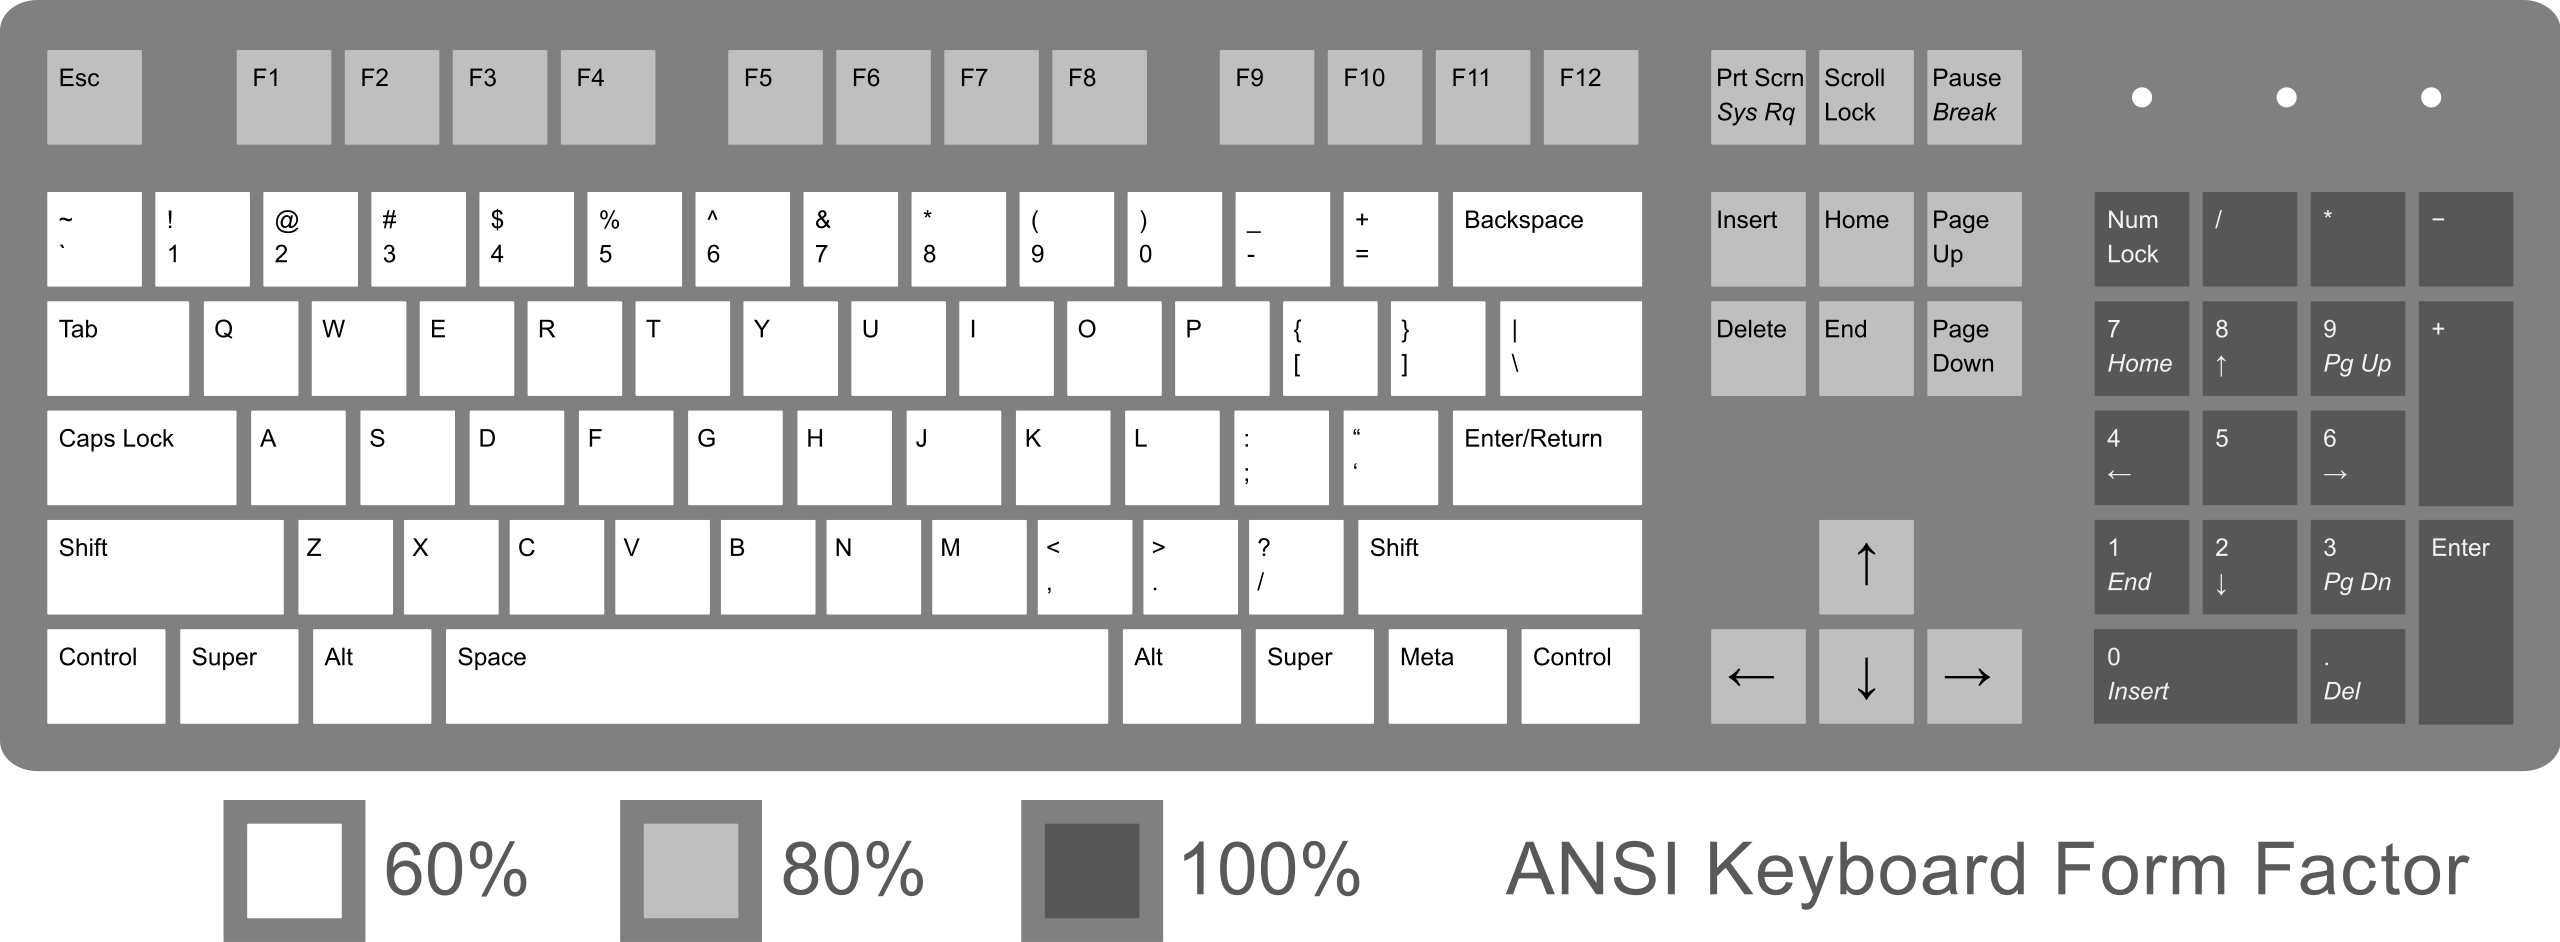
\includegraphics[width=0.8\textwidth]{ansi.png}
	\caption{\ac{ansi} Keyboard layout with form factors. Reprinted from \fullcite{figure-ansi}}
	\label{fig:ansi}
	\centering
\end{figure}

\subsubsection{Ergonomic Keyboards Layouts and Form Factors}

There have been other keyboard layouts and form factors created to mitigate
common issues associated with QWERTY layouts. These include Colemak, Dvorak, and
Alphabetical layouts. However, studies have shown that the layout itself does
not matter as beginners do not necessarily see the keyboard as a structured set,
but rather as a random collection of characters, even if it is alphabetized
\parencite{norman1982},

A different form factor has a great effect on ergonomics. One such example of a
form factor is an ergonomic keyboard developed by Microsoft called Microsoft
Natural MultiMedia Keyboard. \citeauthor{ripat2010} used this keyboard in
determining that ergonomic keyboards can help in reducing symptoms of \ac{neck}.
Figure~\ref{fig:mn} shows the layout of the Microsoft Natural MultiMedia
Keyboard.

\begin{figure}[H]
	\centering
	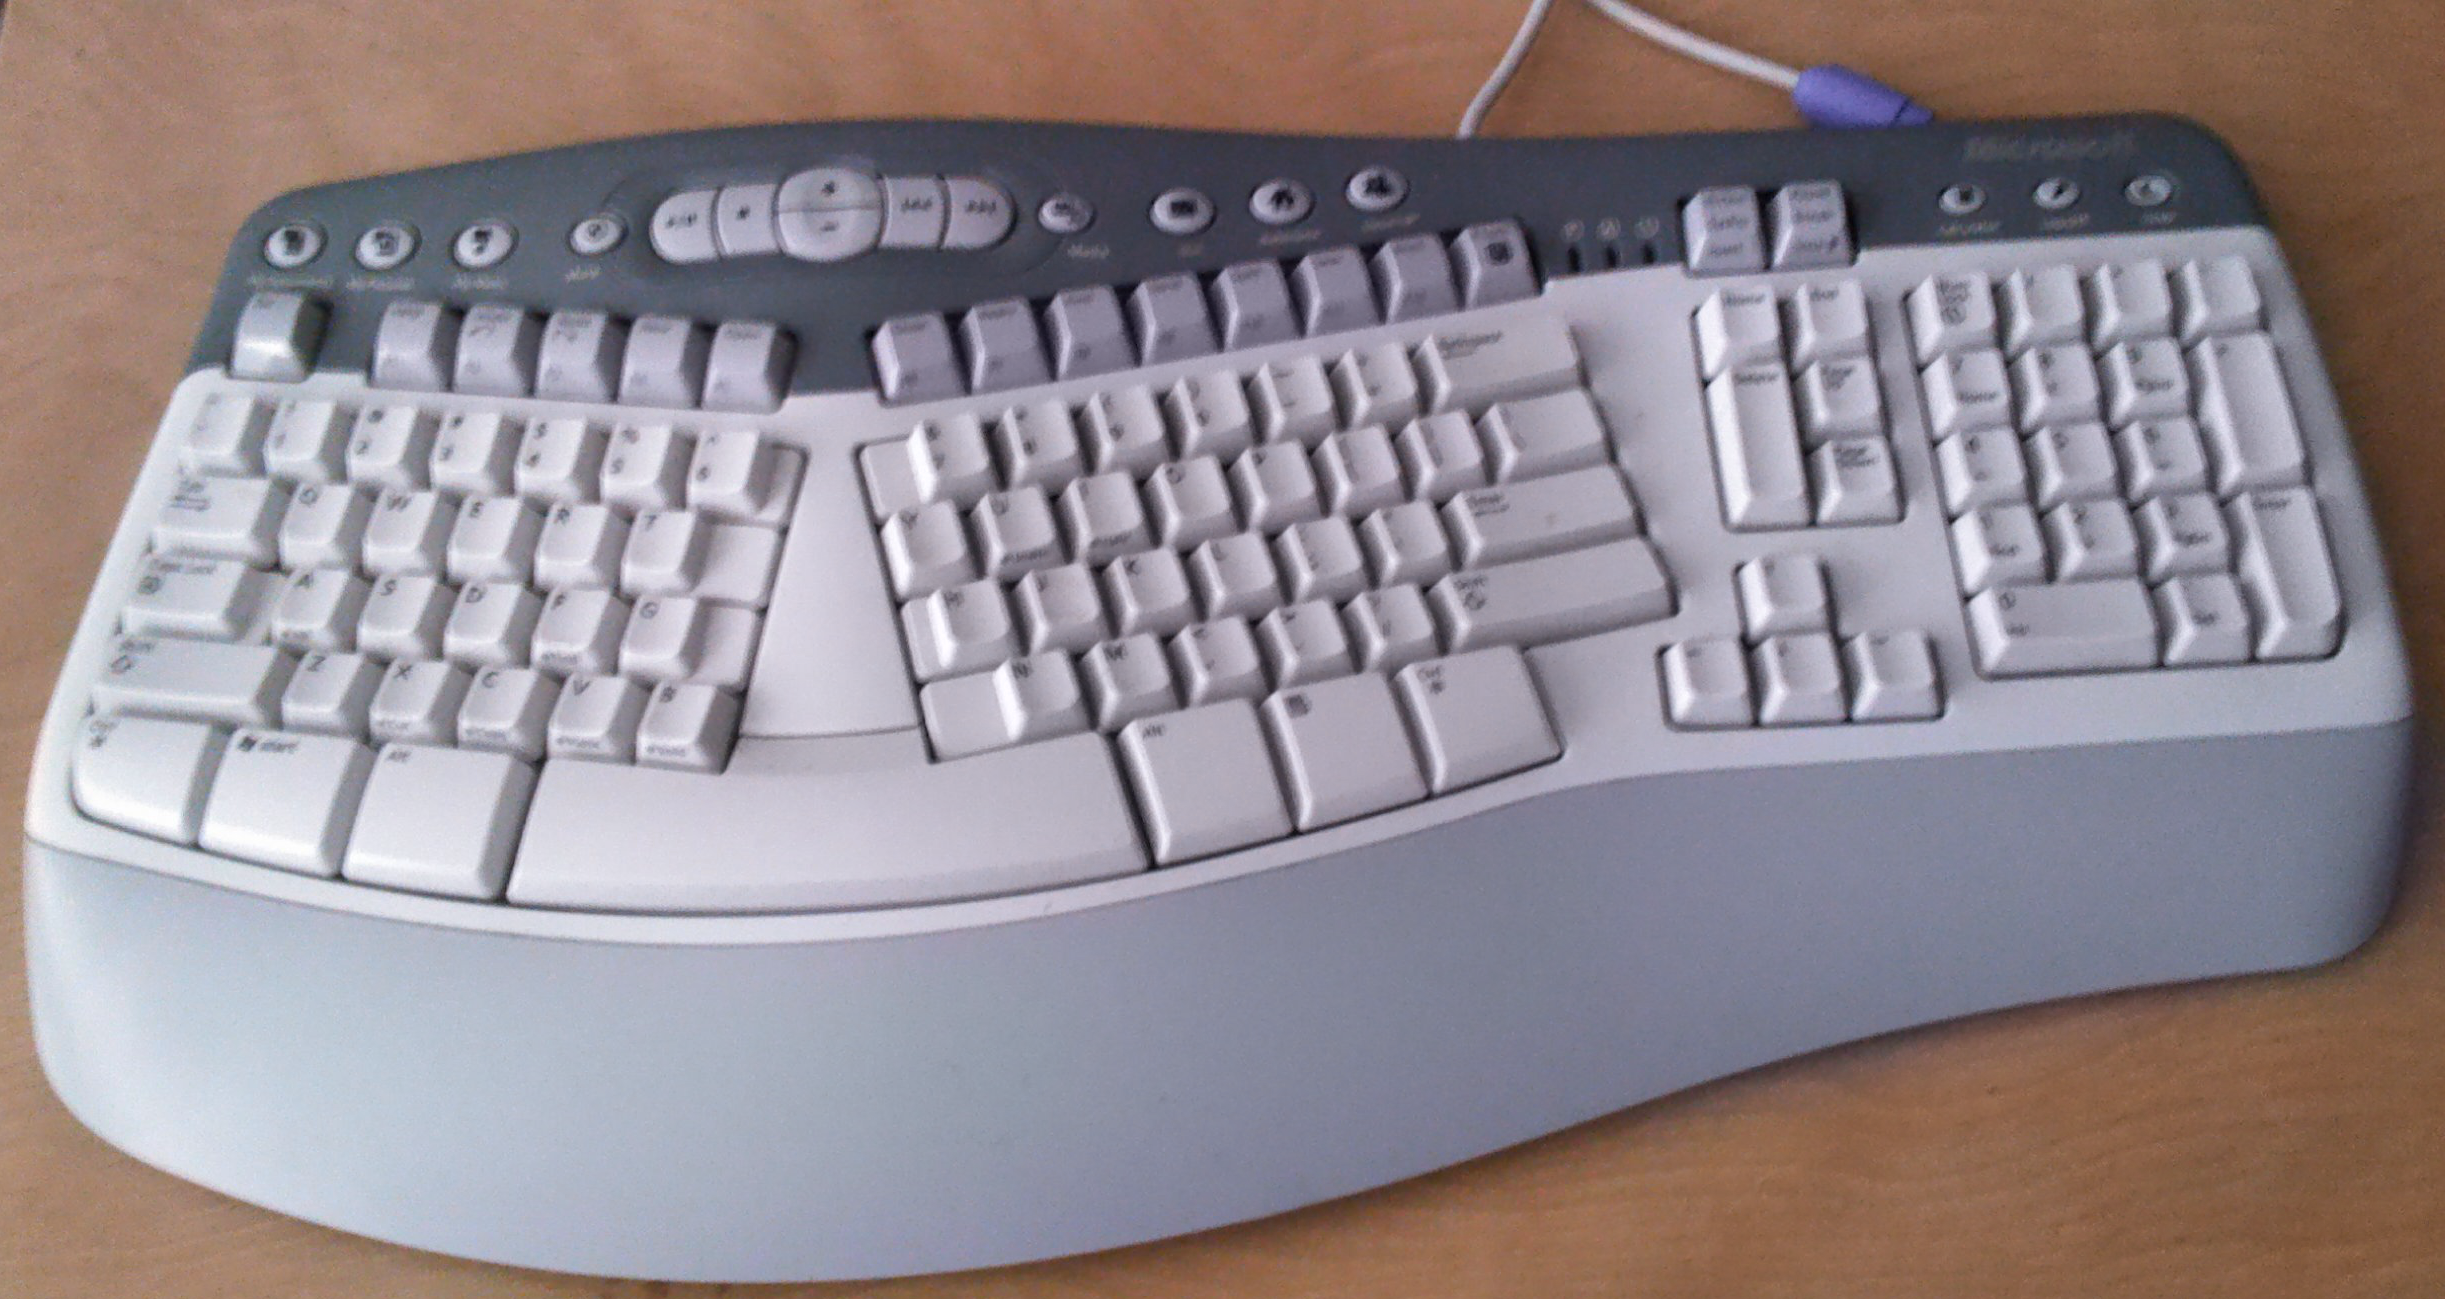
\includegraphics[width=0.8\textwidth]{mn.png}
	\caption{Microsoft Natural MultiMedia Keyboard. Reprinted from \fullcite{mn}}
	\label{fig:mn}
	\centering
\end{figure}

There are other form factors other than the full-size keyboard and variations
thereof that focus on ergonomics. One such example is a split keyboard layout
where the keyboard is split in half, one for the left hand and one for the
right. One such benefit, according to \citeauthor{ergodox}, is a more relaxed
position due to typing at shoulder width.

\subsection{Keyboard Typing Metrics}

There are numerous metrics used to quantify keyboard typing performance. Two
common metrics used in the majority of typing tests include Accuracy and Speed.

\subsubsection{Standardized Keyboard Typing Assessments}

To be able to measure these metrics, a keyboard typing assessment needs to be
done. However, there are no standardized keyboard typing assessments
\parencite{donica2018}. As such, teaching methods and assessments, like
Keyboarding without Tears, Monkeytype, and Keybr, may produce different metrics
for the same typist due to their difference in conducting the assessment.

\subsubsection{Speed}
Speed, also called as entry rate by \citeauthor{arif2009}, measures the number
of characters entered in a specific time frame. The most common metric that
measures speed is \ac{wpm}. \ac{wpm} as defined by \citeauthor{arif2009} is:

\begin{equation}
	WPM = \frac{|T| - 1}{S} \cdot 60 \cdot \frac{1}{5}
\end{equation}

where, $|T|$ is the length of the text, $S$ is the time in seconds spent writing
the text. This time starts directly after the first character has been pressed,
and ends when the last letter has been entered. As such, $1$ is subtracted from
$|T|$, as the time spent to find and press the first character cannot be
accurately determined. However, some typing assessments do not subtract $1$ from
$|T|$. $60$ refers to the number of seconds in a minute and $\frac{1}{5}$
normalizes the metric for the average length of words.


Other metrics also measure speed but they aren't as commonly used as \ac{wpm}.
These include Characters per Minute, Gestures per Second, Adjusted Words per
Minute, and Keystrokes per Second

\subsubsection{Accuracy}
Accuracy measures the number of correctly pressed characters in an input string.
Accuracy, as defined by \citeauthor{bartnik2021}, is:

\begin{equation}
	ACC = \frac{|C|}{|T|} \cdot 100\%
\end{equation}

where $|C|$ is the number of correct characters and $|T|$ is the length of the
text.

The inverse of accuracy is error rate, where the number of incorrectly pressed
characters is measured instead. \citeauthor{arif2009} describe 5 common error
rate metrics: Error Rate, Minimum String Distance Error Rate, Keystroke per
Character, Erroneous Keystroke Error Rate, and Total Error Rate.

\subsubsection{Limitations of the Metrics}
These metrics are all based on the inputted characters by the user. These
metrics do not take into account other aspects of keyboard typing such as
posture, hand and wrist positions, and finger placement. Consequently, these
metrics do not give a full picture of the performance of the person typing and
they only provide a cursory view of how a person types.

\subsection{Keyboard Typing Methodology}
Keyboard typing can be accomplished in numerous ways. The main difference
between the different methodologies is the number of fingers used when typing
and how the typist navigates the keyboard to find the keys. The methodology
ranges from Hunt and Peck to Touch Typing, with variations of the two in
between.

Hunt and Peck uses one finger on one hand to press a key. This method is aided
by using vision to locate the specific key to press \parencite{hoot1986}. On the
other hand, Touch typing uses standard QWERTY mapping to type without using
visual cues. \parencite{dobson2009touch} This mapping involves assigning certain
fingers to certain keys. Figure~\ref{fig:touch-type} is the standard QWERTY
mapping used for an \ac{ansi} layout. Kinesthesis and proprioception are used in
locating the keys \parencite{logan2016}.

\begin{figure}[H]
	\centering
	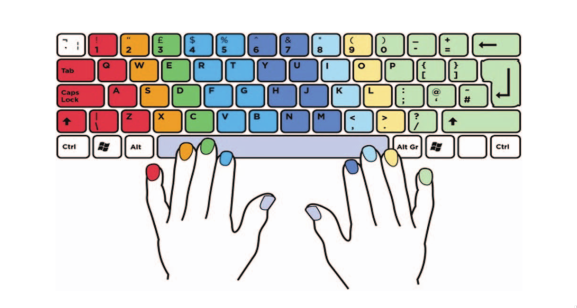
\includegraphics[width=0.8\textwidth]{touch-type.png}
	\caption{Standard QWERTY mapping for \ac{ansi}. Reprinted from \fullcite{logan2016}}
	\label{fig:touch-type}
	\centering
\end{figure}


\section{Keyboard Typing in Education}

Today, students are expected to type essays, articles, and other submissions
using word processors \parencite{poole2016}. Testing is also commonly done using
computerized assessments which require the need for keyboards
\parencite{moodle}. As such, there is a need for students to be well versed in
keyboard typing and for keyboard typing to be part of the curriculum.

Keyboard typing has been a part of this curriculum for a long time, with studies
about effective methods to teach keyboard typing reaching as far back as 1986
\parencite{hoot1986}. Studies have continued to this day to continue to optimize
and improve methods of teaching keyboard typing to students.

These studies start teaching kids in the kindergarten level and the studies try
to optimize the teaching methods to improve the speed and accuracy of typing of
the learners. By starting to teach touch typing to students early, these
students will develop the potential for higher-level keyboard typing
\parencite{donica2018}.

\subsection{Expectations of Keyboard Proficiency}

In the United States, keyboard typing is an expected learning outcome for third
grade in the Common Core State Standards \parencite{ccs}. At this grade level,
only basic keyboard typing skills are required. By fourth grade, students are
expected to have enough proficiency to type one page in one sitting. This is
increased to two pages by fifth grade.

In the Philippine context, the \citeauthor{deped} expects learners with a mental
age of 4--6.9 years old to use correct posture and locate characters, learners
with a mental age of 7--11.9 are introduced to home row finger placement, and
learners with a mental age of 12 and above are expected to ``use proper typing
technique with efficiency and accuracy without looking at the keyboard''
\parencite{deped}.

\subsection{Current Teaching Methods}

Current teaching methods involve replicating a given text. Learners then copy
the text into a given text field that records the typed characters. Correct and
incorrect characters are then identified, and suitable errors are presented.
Afterward, metrics, such as \ac{wpm}, and accuracy are given
\parencite{bartnik2021, typeracer}.

Through this process, the learner goes through the three stages of Motor
Learning Theory. The student undergoes the cognitive stage where they try to
understand and create strategies to accomplish the given task. Then the
associative stage follows where the strategies and skills learned from the
previous stage are refined. At this stage, the learners are expected to rely less
on visuals to locate the keys and more on kinesthesis. By the final stage, the
autonomous stage, the learner does not rely on visuals at all and focuses on
using kinesthetic feedback to find the keys. By this point, the learner has
progressed from using Hunt and Peck, to becoming proficient in touch typing.
\parencite{donica2018}

\subsubsection{Keyboarding without Tears}

Keyboarding without Tears is a web-based application and curriculum that teaches
students touch typing. However, one key differentiator of this curriculum is the
usage of a row-based standard mapping, rather than a column-based standard
mapping that is common in other teaching guides. Figure~\ref{fig:kwt} shows the
standard mapping used in this curriculum.

This curriculum is self-directed and learners can learn at their own pace. At
its core, the curriculum is designed to be 36-week long with 5-10 minutes of
lessons per day. The lessons in the curriculum follow the three stages of
Motor Learning Theory \parencite{kwt}.

\begin{figure}[H]
	\centering
	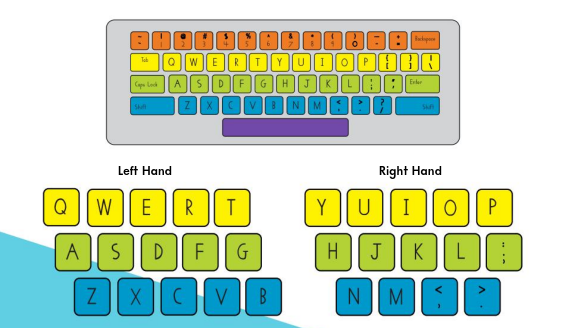
\includegraphics[width=0.8\textwidth]{kwt.png}
	\caption{Row based standard mapping. Reprinted from \fullcite{kwt}}
	\label{fig:kwt}
	\centering
\end{figure}


\subsubsection{Monkeytype, Typeracer}

These two keyboard typing tests are similar. They follow a common experience
where users type a predetermined phrase, quote, or random words, and metrics are
given after the test. Afterward, the learners may try the test again, or choose
another set of words to type. These typing tests do not have a structured
curriculum for learning how to touch type. It is left to the learner to practice
and learn on their own \parencite{bartnik2021, typeracer}.

\subsubsection{Keybr}

Keybr is similar to Monkeytype and Typerace, in that they also have the users
type a predetermined phrase, quote, or random words. However, this application
has more guidance compared to the two. Keybr uses statistics to create typing
lessons that are appropriate to the current typing proficiency of the learner.
The words selected are random at first, and the skill level of the learner is
determined by the performance of the user with these words and characters. The
information gathered is then used to generate new words for the next iteration.
As an example, if a learner has difficulty in typing the letter q, the next
iterations will have a lot of words that contain the letter q.

Statistics from their website show that this learning method is successful, with
some learners improving their typing speed by 20--40 \ac{wpm} \parencite{keybr}.

\section{Keyboard Typing in Health}

There have been a lot of studies that show the effect of keyboard typing, and
its associated movements (or lack thereof), has an effect on the human body.
These studies have shown that keyboard typing has an effect on our neck, shoulder,
upper limb, wrist, arms, and fingers \parencite{szeto2005, baker2007digit}

\subsection{Health Issues arising from Keyboard Typing}

\ac{neck} are a common issue that is associated with an elongated length of time
maintaining a static posture. When using the computer, the posture commonly
adapted by users has the neck and shoulder regions in a static hold for a long
time. This results in forward neck flexion and increased muscle tension
\parencite{szeto2005}.

In addition, it has been shown that 22\% of computer users sustain
musculoskeletal disorders of the upper extremity. This includes the neck,
shoulder, hands, and wrists. \parencite{gerr2002}

Carpal tunnel syndrome is also a common issue in the general population. This is
caused by the chronic compression of the median nerve. There is a common belief
that typing is one main cause for the disorder \parencite{carpal-myth}. There
are no definite conclusions if this myth is true, however, a study by
\citeauthor{toosi2015} found that typing causes ulnar deviation, especially if
done without proper form. This ulnar deviation contributes to the swelling of
the median nerve during and after typing. However, the authors noted that it is
unclear if this swelling leads to long-term nerve injury.

\subsection{Finger and Wrist Kinematics}
The way people move their hands, wrists, and fingers differ between each person.
This can be attributed to the different typing styles each person has. One key
difference between people is the angle of the 5th digit.

However, there are some common movements and positions regardless of typing
style: flexion, or the curving of the fingers, across the fingers, is decreasing
across the hand, with the 2nd digit having the least flexion. This may be due to
the instinct to reduce pronation of the hand, which in turn increases the
distance of the 2nd digit to the keyboard. In addition, some people isolate or
extend one of their thumbs, usually the one not used for pressing a key. This is
also true for some people that do not use their 5th digit during typing
\parencite{baker2007}.

The movement and angle of the wrists also depend on the typing style of the
typists. Some people do not reposition their hands, while others do. This
difference comes from the way these people reach for certain far-away keys. Some
stretch their fingers to reach far-away keys, while others move their entire
hand to reach these keys.

For those that reach their keys by stretching their fingers, there is an
increased probability that the wrists and fingers adapt non-neutral postures.
These include wrist extension, ulnar deviation, and pronation, which may cause
musculoskeletal disorders of the upper extremity (\cite{marklin1999} as cited in
\cite{baker2007})

\section{Finger and Hand Tracking}
Finger and Hand tracking is a method of tracking fingers and hands in 3D space
using motion capture systems or computer vision. This technique allows computers
to perform actions and analyses on the motions and positions of these body
parts.


\subsection{Types of Tracking}

\subsubsection{Hardware Aided Solutions}

Motion Capture Systems allow for capturing detailed skeletal motion in humans.
These systems usually capture full-body motion, focusing on large parts of the
human body, such as the torso, limbs, and head.

However, motion capture systems have difficulty in tracking more articulated
body parts --- with the fingers being one of them. The industry standard for
capturing finger movements is through the use of an optical marker-based motion
capture system. This is due to its ability to capture natural motion accurately.

This method uses cameras to triangulate the 3D location of markers attached to
the limbs of a person. For finger tracking, 13--20 markers are placed on the
fingers, and cameras are brought closer to track the small movements of the
finger \parencite{wheatland2015}.

But this method is cost-prohibitive, and cannot handle occlusions well.
\citeauthor{alexanderson2016} present a method for an optical marker-based
motion capture system that can predictably recover from self-occlusion and has a
better performance compared to previously used algorithms, however, the issue of
cost and self-occlusion still persists.

Bend-sensor gloves are also an option for finger tracking. These gloves have
sensors within them that track joint angles in the hand and fingers. One key
differentiator of this solution compared to the others is the removal of
self-occlusion in the data. As such, this is commonly used in sign language, and
gesture recognition due to its accuracy.

However, these gloves need a lot of time to calibrate as cross-coupling of the
sensors proves a problem. Cross-coupling is prevalent because the movement of
one finger also moves other parts of the hand. These movements may cause a
sensor aimed to track a specific movement of a different part of the hand to
inadvertently detect a movement when there should be none
\parencite{wheatland2015}.

\subsubsection{Computer Vision}

At its core, Computer Vision aims to perform tasks that the human visual system
can do \parencite{cern}. This includes object classification, tracking, and
gesture recognition, and face recognition. At the present, most computer vision
systems utilize deep learning algorithms, and convolutional networks to gather
information from an image, or a set of images. One such example of a
convolutional network used in computer vision is Inception by
\citeauthor{szegedy2015} which proposes a convolutional neural network
architecture for object classification and detection.

\subsection{Available CV Solutions for Tracking}

\subsubsection{OpenCV}

OpenCV is an open-source computer vision and machine learning software library
that houses ${\approx2500}$ optimized algorithms. This library is widely used by
companies, researchers, and open source communities that utilize computer vision
and machine learning in their projects. Examples of companies that use OpenCV
include Google, Sony, and Honda.

The library has C++, Python, Java, and Matlab interfaces. The library also supports
Windows, Linux, Android, and macOS, allowing for great developer experience, and
wide deployment capabilities \parencite{opencv}.

\subsubsection{MediaPipe}

MediaPipe is an open-source computer vision framework that allows developers to
create a perception pipeline. This perception pipeline is a directed graph of
calculators. Data passes through the graph as packets and a group of packets
constitute a data stream. As the data passes through the pipeline, the
calculators, produce the desired output.

This framework allows for performant object detection, hand and finger tracking,
human pose detection. The framework also allows for combining multiple features,
by adding them to the graph as calculators. MediaPipe has C++, Python, JS, and
Coral interfaces. It also supports Android and iOS devices
\parencite{mediapipe}.

\subsubsection{MATLAB}
MATLAB is a programming platform for the analysis and designing of systems.
MATLAB is commonly used by engineers and scientists for computational
mathematics \parencite{what-matlab}.

A toolbox offered by MATLAB is the Computer Vision Toolbox that contains
algorithms, and functions for use in the development of computer vision, 3D
vision, and video processing systems. By using the available algorithms in the
toolbox, such as YOLOv2, and ACF, hand detection and gesture recognition is made
possible in the platform \parencite{matlab}.

\subsection{Applications}

There have been multiple applications and products that utilize hand and finger
tracking as their main component.

\citeauthor{dorf2001} presents a use case for finger tracking in augmented
environments. In the paper, interaction in a virtual environment through the use
of gestures. The tracking system uses an optical marker-based motion capture
system where the user wears a glove with retroreflective markers.

\citeauthor{chiang2014} used a Kinect, a 3D sensing device by Microsoft that
uses depth data, to track fingers to play virtual instruments. Virtual Pianos
and Guitars were created and played with reliable and stable tracking.

\citeauthor{yousaf2014} created a virtual keyboard that operates using finger
tracking. The tracking uses the movement of the finger joints as the basis for
selecting which key to press. A camera captures the movement, and the resulting
video stream is used for hand region detection and finger joint localization.
Using probabilistic regional density-based kernel tracking, finger joint
trajectories are gathered. Feature vectors are then interpreted from the
trajectories. These feature vectors are used in logic-based techniques and
Dynamic Bayesian Network for classification, detection, and recognition of
keystrokes.

\section{Summary of the Research Gap}
While there are a lot of applications and curriculum aimed at teaching touch
typing, there is no automated system available that detects if a person uses the
correct finger to press a key.

By having this system, educators can accurately determine if and when a student
is having a hard time typing and if these students will need an intervention to
correct mistakes.

This is also important because certain movements and hand positions will cause
nerve and muscular disorders that will impact the user. By correcting these
problematic movements and hand positions, these disorders can be prevented.

\newpage
\printbibliography[heading=bibintoc,title={References}]{}

\end{document}
